%-------------------------------------STYLES----------------------------------------------------------------%

\documentclass[10pt, xcolor=dvipsnames]{beamer}

%\mode<presentation>
%{
\usetheme{Madrid}
%\setbeamercovered{transparent}
%} 
%\usefonttheme{professionalfonts}
\usecolortheme{beaver}

\usepackage{setspace}
\usepackage[english]{babel}
\usepackage[latin1]{inputenc}
\usepackage{times}
\usepackage[T1]{fontenc}
\usepackage{color}
\usepackage{graphicx}
\usepackage{amssymb}
\usepackage{amsthm}
\usepackage{bm}
\usepackage{rotating}
\usepackage{ccaption}
\usepackage{booktabs}
\usepackage{lscape}
\usepackage{colortbl}
\usepackage{arydshln}
\usepackage{tabularx}
\usepackage{appendixnumberbeamer}

%\useinnertheme{rounded}
\setbeamertemplate{items}[balls]
%\usepackage[notocbib]{apacite}                % This is bibliography package.
%\renewcommand{\bibliographytypesize}{\tiny}
\setbeamertemplate{navigation symbols}{}
\usepackage{graphics}
\usepackage{epstopdf}
\DeclareGraphicsRule{.tif}{png}{.png}{`convert #1 `dirname #1`/`basename #1 .tif`.png}
%\usepackage{fleqn}
%\setlength{\mathindent}{1cm}
%\color{white}
%\hypersetup{colorlinks=true,linkcolor=Blue}
\usepackage{bbm}
\newcommand{\backupbegin}{
   \newcounter{framenumberappendix}
   \setcounter{framenumberappendix}{\value{framenumber}}
}
\newcommand{\backupend}{
   \addtocounter{framenumberappendix}{-\value{framenumber}}
   \addtocounter{framenumber}{\value{framenumberappendix}}
}

%% Change the margins
\newenvironment{changemargin}[2]{%
  \begin{list}{}{%
    \setlength{\topsep}{0pt}%
    \setlength{\leftmargin}{#1}%
    \setlength{\rightmargin}{#2}%
    \setlength{\listparindent}{\parindent}%
    \setlength{\itemindent}{\parindent}%
    \setlength{\parsep}{\parskip}%
  }%
  \item[]}{\end{list}}

\newtheorem{proposition}{Proposition}

%-------------------------------------------Title---------------------------------------------------%


\title[Land Constraints]{{How Tight are Malthusian Constraints?}}

\author[Johnson \& Vollrath]{T. Ryan Johnson \inst{1} \and Dietrich Vollrath \inst{2}}
\institute[UH]{\inst{1} University of Houston \and %
                      \inst{2} University of Houston}

\date[May 2017]{}

%-------------------------------------------Slides---------------------------------------------------%

\begin{document}
\maketitle

\section{Introduction}

\begin{frame}{How Tight are Malthusian Constraints?}\label{define}

\begin{itemize}
  \item \textbf{Malthusian constraint}: using a fixed factor (e.g. land) in agricultural production
  \item \textbf{How Tight?}: what is the elasticity of agricultural output w.r.t land?
\end{itemize}

\end{frame}


\begin{frame}{In this paper}
Estimate the elasticity of agricultural output w.r.t land
\begin{itemize}
  \item Use relationship of \textit{rural} density and agro-climatic agricultural TFP to estimate the elasticity of output w.r.t land
  \item Estimates come from \textit{within}-province variation across districts
  \item Population data from HYDE
  \item Agro-climatic TFP built from Galor and {\"O}zak data on caloric suitability
\end{itemize}

\vspace{.2cm} Advantages of our method
\begin{itemize}
  \item Not assuming elasticity is same \textit{across} or \textit{within} countries
  \item Do not need data on inputs other than land or labor
\end{itemize}

\end{frame}

\begin{frame}{In this paper}
We find:
\begin{itemize}
  \item Elasticities range from 0.1 to 0.3, vary by region
  \item Variation is related to agro-climatic conditions
  \item Temperate, cold, regular rain ($\sim 0.3$) $\Rightarrow$ tight Malthusian constraints
  \item Equatorial, hot, seasonal rain ($\sim 0.1$) $\Rightarrow$ loose Malthusian constraints
\end{itemize}

\end{frame}

\begin{frame}{Implications}
Elasticity determines degree of decreasing returns to mobile factors in agriculture

\vspace{.2cm} Higher elasticity $\Rightarrow$
\begin{itemize}
  \item more sensitive $L_A/L$ is to TFP or population shocks
  \item more sensitive $y$ is to TFP or population shocks
\end{itemize}

\vspace{.2cm} Variation in elasticity informative for
\begin{itemize}
  \item effect of Black Death on Europe? 
  \item source of ``involution'' in Asia?
  \item slow development of tropical areas?
\end{itemize}

\end{frame}

\begin{frame}{Some Related Literature:}
\begin{itemize}
  \item \textbf{Geography and development:} Olsson and Hibbs (2005); Ashraf and Galor (2011); Nunn and Qian (2011); Nunn and Puga (2012); Michalopoulos (2012); Alesina, Giuliano, Nunn (2013); Cook (2014a,b); Fenske (2014); Alsan (2015); Ashraf and Michalopoulos (2015); Dalgaard, Knudsen, Selaya (2015); Galor and {\"O}zak (2016); Litina (2016); Andersen, Dalgaard, Selaya (2016); Frankema and Papaioannou (2017)
  \item \textbf{Malthusian and UGT models:} Galor (2011); Galor and Weil (2000); Galor and Moav (2002); Hansen and Prescott (2002); Doepke (2004); Cervellati and Sunde (2005); L{\"a}gerlof (2006); Crafts and Mills (2009); Strulik and Weisdorf (2008), Voigtl{\"a}nder and Voth (2013a,b)
  \item \textbf{Agriculture and development:} Gollin, Parente, Rogerson (2007); Restuccia, Yang, Zhu (2008); Weil and Wilde (2009), Gollin (2010)
  \item Motamed, Florax, Masters (2014): Pattern/date of urbanization at grid-cell level based on agro-climatic conditions
  \item Henderson, Squires, Storeygard, Weil (2016): Spatial organization of economic activity, relationship to geographic conditions
\end{itemize}

\end{frame}

\section{Model}

\begin{frame}{Density and Productivity}
Region $I$ contains a set of districts, each denoted by $i$, with aggregate agricultural production
\begin{equation}
Y_{i} = A_{i} X_{i}^{\beta} \left(K_{Ai}^{\alpha}L_{Ai}^{1-\alpha}\right)^{1-\beta} \label{EQ_production}
\end{equation}
\begin{itemize}
  \item $A_i$ is productivity, $X_i$ is land
  \item $K_{Ai}$ is all other inputs (e.g. capital)
  \item $L_{Ai}$ is agricultural labor in district $i$ (not a single sector)
  \item Assume $\beta$ and $\alpha$ are identical \textit{within} region (but not nec. \textit{across} regions)
\end{itemize}
\end{frame}

\begin{frame}{Mobile Factors}
The wage and return to capital in each district are given by 
\begin{eqnarray}
    w = \phi_L \frac{Y_i}{L_{Ai}} \\ \nonumber
    r = \phi_K \frac{Y_i}{K_{Ai}} \label{EQ_factorprices}
\end{eqnarray}
\begin{itemize}
  \item $\phi_L$ and $\phi_K$ are shares of output 
  \item Shares need not equal elasticities
  \item Shares are identical \textit{within} region (but not nec. \textit{across} regions)
  \item Capital and labor are mobile \textit{within} region (but not nec. \textit{across} regions)
\end{itemize}
\end{frame}

\begin{frame}{Solving for Labor Allocations}
Given mobility of labor and capital within region,
\begin{equation}
    \frac{K_{Ai}}{L_{Ai}} = \frac{w}{r}\frac{\phi_K}{\phi_L}.
\end{equation}
Adding up condition for agricultural labor within region
\begin{equation}
\sum_{i\in I} L_{Ai} = L_A.
\end{equation}
Solve for allocation of labor (relative to land) to district $i$
\begin{equation}
\frac{L_{Ai}}{X_i} = A_{i}^{1/\beta}\frac{L_A}{\sum_{j\in I} A_{j}^{1/\beta}X_{j}}. \label{EQ_LaX}
\end{equation}
\end{frame}

\begin{frame}{Agricultural Labor Allocation}
Take logs of $L_{Ai}/X_i$ expression
\begin{equation}
\ln L_{Ai}/X_i = \frac{1}{\beta} \ln A_{i} + \ln \Gamma, \label{EQ_est}
\end{equation}
where
\begin{equation}
    \Gamma = \frac{L_A}{\sum_{j\in I} A_{j}^{1/\beta}X_{j}}.
\end{equation}
is a \textit{region-specific} term. 

\begin{itemize}
  \item $\beta$ can be estimated from elasticity of $L_{Ai}/X_i$ w.r.t. $A_i$. 
  \item $1/\beta$ small (tight), ag. workers spread evenly w/in region
  \item $1/\beta$ large (loose), ag. workers concentrated on high $A_i$
\end{itemize}
\end{frame}

\begin{frame}{Agricultural Labor Allocation}\label{model}
Take logs $L_{Ai}/X_i$ expression
\begin{equation}
\ln L_{Ai}/X_i = \frac{1}{\beta} \ln A_{i} + \ln \Gamma, \label{EQ_est}
\end{equation}
where
\begin{equation}
    \Gamma = \frac{L_A}{\sum_{j\in I} A_{j}^{1/\beta}X_{j}}.
\end{equation}
is a \textit{region-specific} term. 

\begin{itemize}
  \item $\Gamma$ is constant for all districts w/in region
  \item Ag labor relative to total labor ($L_A/L$) does not enter
  \item Expression is not unique to heaviliy agricultural regions (or eras)
\end{itemize}

\hfill \hyperlink{extend}{\beamerbutton{More}}
\end{frame}

\section{Regression Setup}

\begin{frame}{A simple example, 1500CE}
Slopes indicate size of $1/\beta$:
\begin{center}
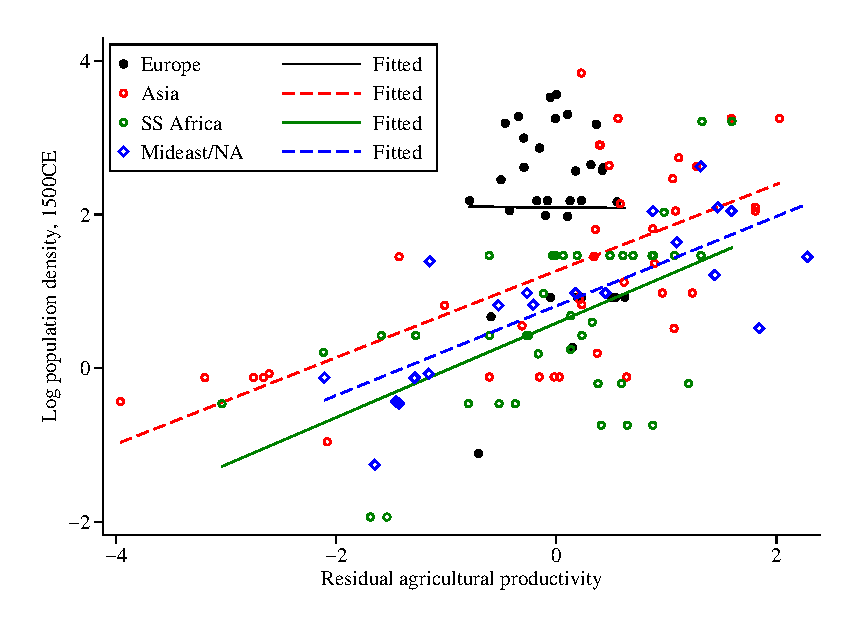
\includegraphics[width=.75\textwidth]{fig_ag_regions.eps}
\end{center}
{\scriptsize Data from Ashraf and Galor (2010). Residual plot using their controls except continent FE.}
\end{frame}

\begin{frame}{Using as a Specification}
Re-arranging the prior expression and adding some notation:
\begin{equation}
  \ln A_{isc} = \alpha + \beta \ln L_{Aisc}/X_{isc} + \gamma_{sc} + \delta' \mathbf{Z}_{isc} + \epsilon_{isc}. \label{EQ_regress}
\end{equation}

\begin{itemize}
  \item District $i$, region/state/province $s$, country $c$
  \item $\gamma_{sc}$, region/country FE, pick up $\Gamma$ term
  \item $\mathbf{Z}_{isc}$ are additional controls
  \item $\epsilon_{isc}$ is error term
\end{itemize}
\end{frame}

\begin{frame}{Using as a Specification}
We moved productivity, $A_{isc}$ and agric. density $L_{Aisc}/X_{isc}$ to opposite sides:
\begin{equation}
  \ln A_{isc} = \alpha + \beta \ln L_{Aisc}/X_{isc} + \gamma_{sc} + \delta' \mathbf{Z}_{isc} + \epsilon_{isc}. \label{EQ_regress}
\end{equation}

\begin{itemize}
  \item Not a causal statement
  \item Estimating $1/\beta$ $\Rightarrow$ SE's on $\beta$ explode
\end{itemize}
\end{frame}

\begin{frame}{Agricultural Density Data}
$L_{Aisc}$ comes from HYDE 3.1 database (Goldewijk et al, 2011)
\begin{itemize}
  \item Population counts for 5 degree grid-cells built from administrative data
  \item We aggregate data back to administrative level (e.g. districts)
  \item Rural population data (not agricultural)
  \item Main samples based on year 2000
\end{itemize}
$X_{isc}$ calculated as area of a given district
\begin{itemize}
  \item Overstates size of agricultural land
\end{itemize}
$L_{Aisc}/X_{isc}$ data 
\begin{itemize}
  \item Trim above 99th and below 1st percentiles
  \item Drop if fewer than 100 total rural residents
  \item 32,862 total districts
\end{itemize}
\end{frame}

\begin{frame}{Agricultural Density Data}
\begin{center}
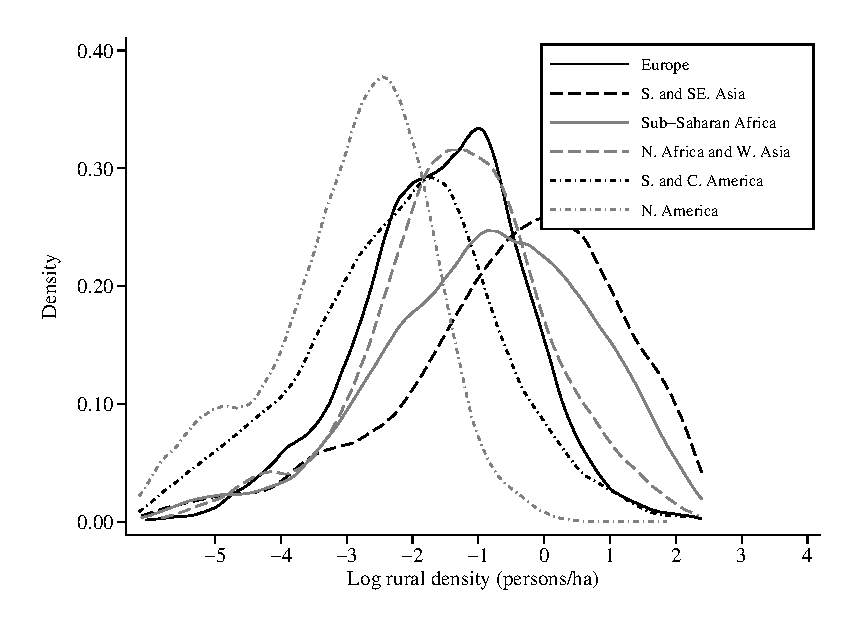
\includegraphics[width=.8\textwidth]{fig_dens_rurd.eps}
\end{center}
\end{frame}

\begin{frame}{Agricultural Density Data}
\begin{center}
\includegraphics[scale=.5]{fig_rurd_map.png}
\end{center}
\end{frame}

\begin{frame}{Agricultural Productivity Data}\label{data}
$A_{isc}$ is built similar to Galor and {\"O}zak (2016) caloric suitability index
\begin{itemize}
  \item Data from GAEZ on agro-climatic possible yield (in raw tons) for each crop
  \item Combine with nutritional information by crop (total calories per raw ton)
  \item For each grid cell, determine max calories across crops
  \item Total max calories across grid cells in district, divide by total area
  \item As in Galor and {\"O}zak, holds technology assumptions constant
  \item Trim above 99th and below 1st percentile
\end{itemize}
\hfill \hyperlink{stats}{\beamerbutton{Summary}}

\hfill \hyperlink{crops}{\beamerbutton{Crops}}
\end{frame}

\begin{frame}{Agricultural Productivity Data}
\begin{center}
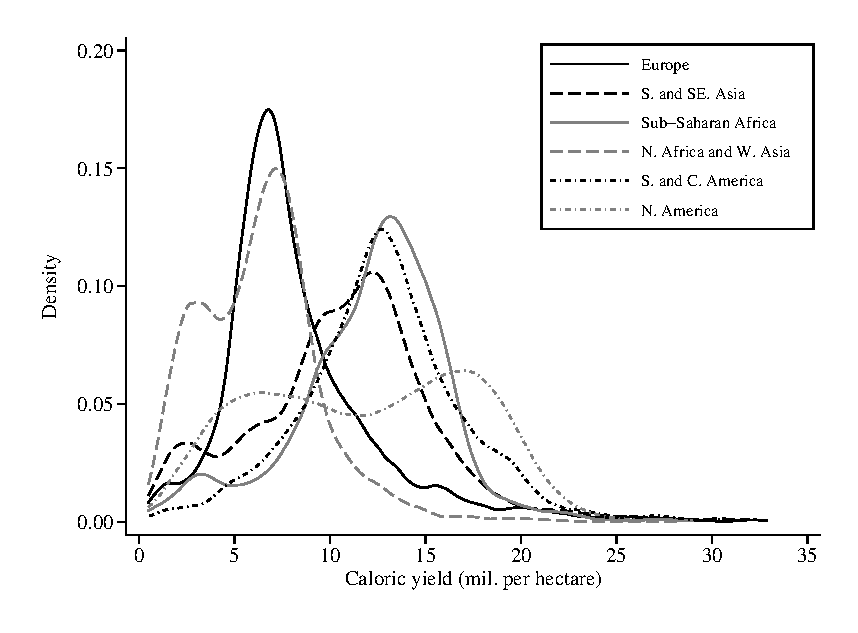
\includegraphics[width=.8\textwidth]{fig_dens_csi.eps}
\end{center}
\end{frame}

\begin{frame}{Agricultural Productivity Data}
Grid cells take values of their district. Shown by percentiles.
\vspace{-.5in}
\begin{center}
\includegraphics[scale=.5]{fig_csi_yield_map.png}
\end{center}
\end{frame}

\begin{frame}{Control Variables}
Henderson et al (2016) on spatial distribution of economic activity
\begin{itemize}
  \item Urban activity correlated with (caused by?) high agricultural productivity (in some places)
  \item Low rural density because of urban activity
  \item $Corr(\epsilon_{isc},\ln L_{isc}/X_{isc})<0$
\end{itemize}

Include two controls at the district level in $\mathbf{Z}_{isc}$ for urban/economic activity:
\begin{itemize}
  \item Night lights density: follows Henderson et al (2016) using Global Radiance Calibrated data
  \item Urban percent of population: from HYDE
\end{itemize}

\end{frame}

\begin{frame}{Spatial Errors and Hypothesis Testing}\label{testing}
Assume $\epsilon_{isc}$ has spatial auto-correlation. Use Conley s.e. (500km window). 

\vspace{.2cm} Two hypothesis tests:
\begin{itemize}
  \item Is the land constraint binding? 
    \begin{itemize}
      \item $H_0: \beta=0$ vs. two-sided alt 
    \end{itemize}
  \item Is the land constraint the same in two samples (e.g. Europe and Sub-Saharan Africa)? 
    \begin{itemize}
      \item $H_0: \beta = \beta^{Ref}$ vs. two-sided alt 
      \item $\beta^{Ref}$ from ad hoc ``reference'' sample
      \item Implemented with interaction regression combining given and reference sample
    \end{itemize}
\end{itemize}
\hfill \hyperlink{interaction}{\beamerbutton{Interaction}}
\end{frame}

\section{Results}

\begin{frame}{Results by Major Region}\label{region}
\begin{center}
\includegraphics[width=.8\textwidth]{fig_coef_region.eps}
\end{center}
\hfill \hyperlink{regiontab}{\beamerbutton{Table}}
\end{frame}

\begin{frame}{Results by Sub-Region}\label{subregion}
\begin{center}
\includegraphics[width=.8\textwidth]{fig_coef_subregion.eps}
\end{center}
\hfill \hyperlink{subregiontab}{\beamerbutton{Table}}
\end{frame}

\begin{frame}{Results for China, Japan, Korea}\label{china}
\begin{center}
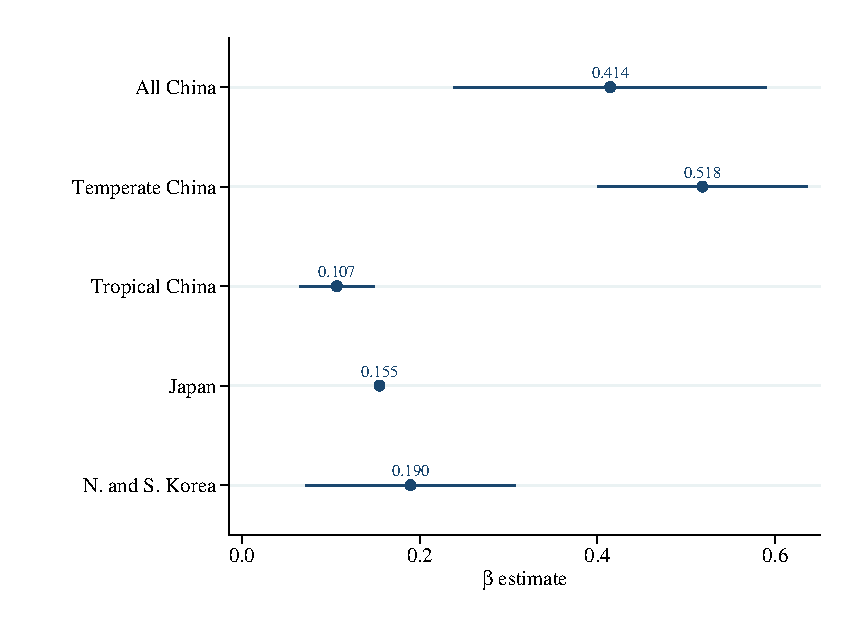
\includegraphics[width=.8\textwidth]{fig_coef_china.eps}
\end{center}
\hfill \hyperlink{chinareg}{\beamerbutton{Table}}
\end{frame}

\begin{frame}{Results by Crop}
Region and sub-region results appear correlated with agro-climatic zones:
\begin{itemize}
  \item Samples based on GAEZ suitability indices for each crop (0 to 100)
  \item Index is based purely on climate and soil characteristics
  \item Include districts using 0 vs $>0$ suitability
  \item $\Rightarrow$ heterogeneity within countries in $\beta$
  \item Not estimating a crop-specific production function
\end{itemize}
\end{frame}

\begin{frame}{Results by Crop}
\begin{center}
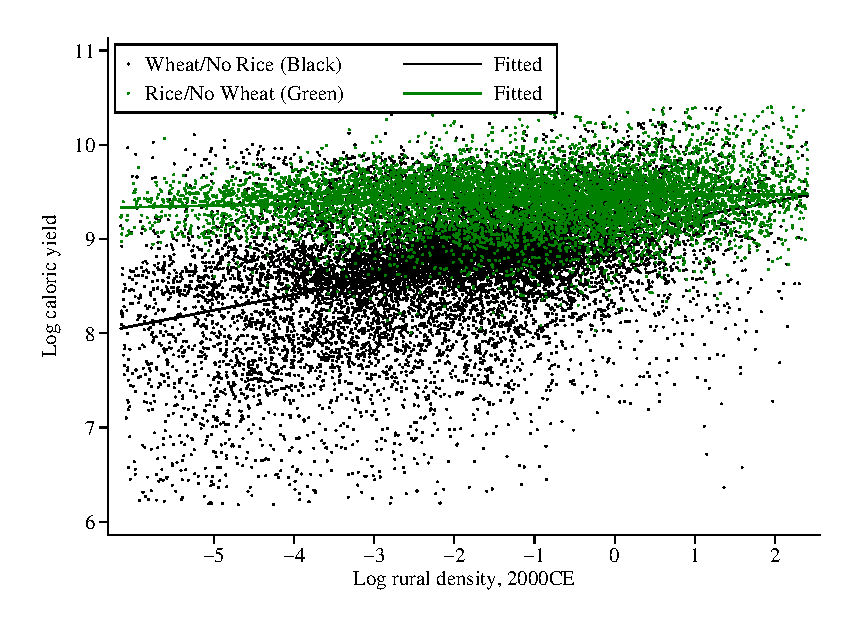
\includegraphics[width=.8\textwidth]{fig_beta_crop.eps}
\end{center}
\end{frame}

\begin{frame}{Results by Crop}\label{crop}
\begin{center}
\includegraphics[width=.8\textwidth]{fig_coef_crop.eps}
\end{center}
\hfill \hyperlink{cropreg}{\beamerbutton{Table}}
\end{frame}

\begin{frame}{Results by Climate Zone}
Crop suitability based in part on climate conditions. 
\begin{itemize}
  \item Create samples based on K{\"o}ppen-Geiger zones
  \item Three layers: Climate, Precipitation, Temperature
  \item Each layer has multiple types (e.g. Climate is Equatorial, Arid, ...)
  \item Create samples where districts have >50\% of land in a given type
  \item $\Rightarrow$ heterogeneity within countries in $\beta$  
\end{itemize}
\end{frame}


\begin{frame}{Results by Climate Zone}\label{climate}
\begin{center}
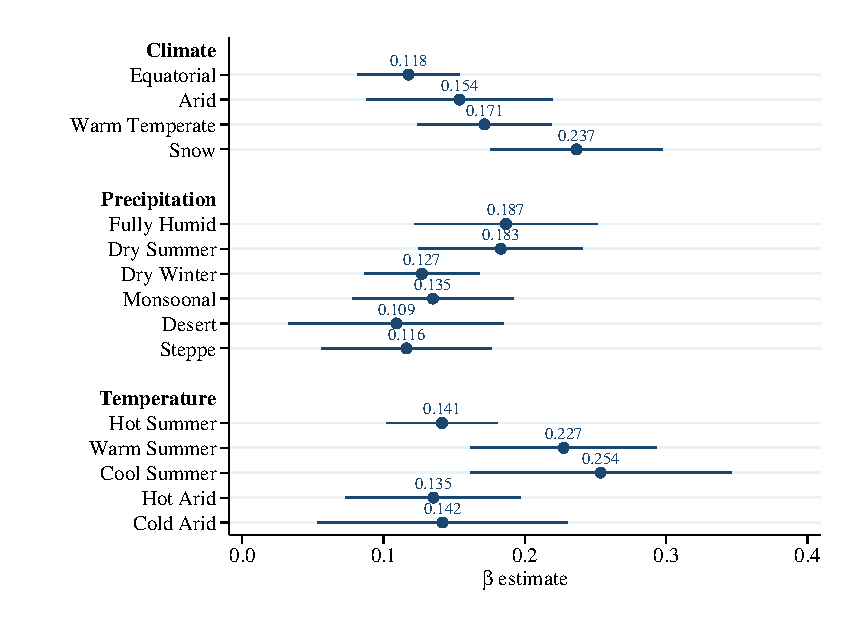
\includegraphics[width=.8\textwidth]{fig_coef_kg.eps}
\end{center}
\hfill \hyperlink{climatereg}{\beamerbutton{Table}}
\end{frame}

\begin{frame}{Explanations?}
Evidence suggests:
\begin{itemize}
  \item Tight constraints: temperate/snow, fully humid/dry summer, warm/cool summers
  \item Loose constraints: equatorial/arid, dry winter/monsoon, hot summer/arid
\end{itemize}

\vspace{.2cm} Why looser constraints in ``tropics''?
\begin{itemize}
  \item Positive(?): Multiple cropping, longer growing periods, more sun, more rain during growing periods $\Rightarrow$ land area isn't binding?
  \item Negative(?): Soil leaching, lack of frost $\Rightarrow$ land is less useful?
\end{itemize}
\end{frame}


\begin{frame}{Robustness}\label{robustness}
\begin{itemize}
  \item Use province level data (with country FE) \hyperlink{regprov}{\beamerbutton{Results}}
  \item Use rural density from 1900 from HYDE \hyperlink{reg1900}{\beamerbutton{Results}}
  \item Use untrimmed samples of rural density and/or agricultural productivity
  \item Use districts with fewer than 100 rural residents
  \item Clustered standard errors (at province level) \hyperlink{cluster}{\beamerbutton{Results}}
  \item Estimate $\beta$ for individual provinces \hyperlink{prov}{\beamerbutton{Results}}
  \item Workers not mobile between districts? \hyperlink{nonmobile}{\beamerbutton{Results}}
  \item Districts autarkic? \hyperlink{autarky}{\beamerbutton{Results}}
\end{itemize}
\end{frame}

\begin{frame}{Measurement Error}
Measurement error $\Rightarrow$ attentuation bias
\begin{itemize}
  \item Population data from HYDE may not be accurate for districts
  \item Is measurement error more pronounced in some regions (e.g. SE Asia) and driving results?
  \item Is true variance of $\ln L_{Aisc}/X_{isc}$ one-third of measured variance?
  \item Is rural population mis-stated by factor of $>2$ or $<0.5$?
\end{itemize}
\end{frame}

\begin{frame}{Measurement Error}
Measurement error of land area, $X_{isc}$
\begin{itemize}
  \item We are using total land area, not cultivated area, so $X_{isc}$ always overstated
  \item Systematic mismeasurement of districts within a province not a problem
  \item Variation in systematic mismeasurement across provinces not a problem
  \item Problem is \textit{variation in noise of mismeasurement} across provinces
  \item Some provinces have more geographic noise across districts?
\end{itemize}
\end{frame}

\begin{frame}{Cultivated area}\label{cult}
Cultivated area, $X^C_{isc}$, available from GAEZ. Rural density is
\begin{equation}
  \ln L_{Aisc}/X_{isc} = \ln L_{Aisc}/X^C_{isc} + \ln X^C_{isc}/X_{isc}
\end{equation}

\begin{itemize}
  \item Regress $\ln A_{isc}$ on both terms on the right hand-side 
  \item Coefficient on $\ln L_{Aisc}/X^C_{isc}$ gives similar results for $\beta$
  \item Coefficient on $\ln X^C_{isc}/X_{isc}$ is within 0.02 of $\beta$ (excl. S/SE Asia)
\end{itemize}

\hfill \hyperlink{cultreg}{\beamerbutton{Results}}
\end{frame}


\begin{frame}{Elasticity of Substitution?}\label{eos}
What if land and labor do not have elasticity of subs. equal to one?
\begin{itemize}
  \item Elasticity of output w.r.t. land depends on rural density $L_A/X$
  \item With EOS more than one, higher density, lower elasticity
  \item Do results fit this?
  \begin{itemize}
    \item South/SE Asia, some SS Afr are high density, low $\beta$
    \item ..but C/S America, other SS Afr are low density, low $\beta$
    \item ..but N America lowest density, not highest $\beta$
  \end{itemize}
\end{itemize}
\hfill \hyperlink{rurdbeta}{\beamerbutton{Density?}}
\end{frame}


\section{Implications}

\begin{frame}{Back to the model}\label{extend}
Aggregate production of agricultural good
\begin{equation}
    Y_A = A_A \left(\frac{K_A}{L_A}\right)^{\alpha(1-\beta)} L_A^{1-\beta}, \label{EQ_caL_solve}
\end{equation}
where 
\begin{equation}
    A_A = \left(\sum_{j\in I} A_{j}^{1/\beta}X_{j} \right)^\beta \nonumber
\end{equation}
and non-agricultural good
\begin{equation}
    Y_N = A_N \left(\frac{K_N}{L_N}\right)^{\alpha} L_N. \label{EQ_YN}
\end{equation}
\end{frame}

\begin{frame}{Factor shares and mobility}
Land earns zero return
\begin{itemize}
  \item No effect of $\beta$ on factor share
  \item Let $\phi_L$ and $\phi_K$ be factor shares of labor and capital in both sectors
\end{itemize}

\vspace{2mm} Mobility of labor between sectors
\begin{equation}
    p_A \phi_L \frac{Y_A}{L_A} = p_N \phi_L \frac{Y_N}{L_N}. \label{EQ_mobility}
\end{equation}
where $p_A$ and $p_N$ are nominal prices of agric. and non-agric.

\vspace{2mm} Mobility of capital implies $K_A/L_A = K_N/L_N = K/L$.

\end{frame}

\begin{frame}{Preferences}
Following Boppart (2014), there exists a utility function such that
\begin{equation}
    \ln c_A = \ln \theta_A + (1-\epsilon) \ln M + (\gamma - 1) \ln p_A + (\epsilon - \gamma) \ln p_N \label{EQ_ca_demand}
\end{equation}
is the demand for $c_A$.
\begin{itemize}
  \item $\theta_A$ is a preference parameter
  \item $M$ is nominal income
  \item $0 < \epsilon < 1$ to capture Engel's Law
  \item $\epsilon > \gamma$ means willingness to substitute between $c_A$ and $c_N$
\end{itemize}
\end{frame}

\begin{frame}{Solving}
Agricultural labor share is
\begin{equation}
  \frac{L_A}{L} = \theta_A \left(\frac{L^{\beta\gamma}}{A_A^{\gamma} A_N^{\epsilon - \gamma} \hat{k}^{\alpha(\epsilon - \beta\gamma)}}\right)^{\frac{1}{1-\beta\gamma}} \label{EQ_LAL}
\end{equation}
while real income (in agricultural terms, $M/p_A$)
\begin{equation}
  y = \left(\frac{A_A A_N^{\beta(\epsilon-\gamma)}\hat{k}^{\Omega}}{L^{\beta}} \right)^{\frac{1}{1-\beta\gamma}} \label{EQ_y}
\end{equation}
where $\hat{k} = (\phi_K K/\phi_L L)$, and $\Omega = \alpha(1-\beta) + \alpha\beta(\epsilon-\gamma)$
\end{frame}

\begin{frame}{Elasticities}
The elasticities of the agricultural labor share ($L_A/L$) and real income ($y$) with respect to various shocks,
\begin{enumerate}
  \item[(a)] Agricultural productivity ($A_A$): 
\begin{equation}
  \frac{\partial \ln L_A/L}{\partial \ln A_A} = - \frac{\gamma}{1-\beta\gamma} \quad \quad \frac{\partial \ln y}{\partial \ln A_A} = \frac{1}{1-\beta\gamma}
\end{equation}
  \item[(b)] Non-agricultural productivity ($A_N$): 
\begin{equation}
  \frac{\partial \ln L_A/L}{\partial \ln A_N} = - \frac{\epsilon-\gamma}{1-\beta\gamma} \quad \quad \frac{\partial \ln y}{\partial \ln A_N} = \frac{\beta(\epsilon-\gamma)}{1-\beta\gamma}
\end{equation}
  \item[(c)] Population ($L$): 
\begin{equation}
  \frac{\partial \ln L_A/L}{\partial \ln L} = \frac{\beta\gamma}{1-\beta\gamma} \quad \quad \frac{\partial \ln y}{\partial \ln L} = - \frac{\beta}{1-\beta\gamma}
\end{equation}
\end{enumerate}
are all increasing in $\beta$.
\end{frame}

\begin{frame}{Implications}
Three settings where the Malthusian constraint might matter
\begin{itemize}
  \item \textbf{Effect of Black Death:} Large effects on European development (Voigtl{\"a}nder and Voth, 2013a,b) due to tight constraint? Similar epidemics in Asia w/o major changes due to loose constraint?
  \item \textbf{Involution:} Higher densities and output, but not living standards, in response to productivity (Geertz, 1963; Huang, 1990) due to loose constraint?
  \item \textbf{Response to agric. technology/inputs:} Necessary increase to match rich countries in TFP/inputs is larger with loose constraint (Eberhardt and Vollrath, 2016a,b)
\end{itemize}

\end{frame}
\section{Conclusion}

\begin{frame}{Conclusion}
\begin{itemize}
  \item Estimate Malthusian constraint from variation in rural density within provinces
  \item Constraint is ``tight'' (0.20-0.30) in temperate areas (N. China, Europe, US/Canada, S. Africa)
  \item Constraint is ``loose'' (0.10-0.15) in tropical areas (S. China, SE Asia, C. Africa, S/C America)
  \item Constraint dictates the sensitivity of $L_A/L$ and living standards to population and productivity
\end{itemize}
\end{frame}

\section{Appendix Slides}
\appendix

\begin{frame}{Interaction Regression}\label{interaction}
Combine a given sample with the reference sample (denoted by $Ref$). Run the following regression with interaction terms
\begin{eqnarray}
    \ln A_{isc} = \beta \ln L_{Aisc}/X_{isc} + (\beta^{Ref} - \beta) \ln L_{Aisc}/X_{isc} \times I(Ref) \\ \nonumber
    + \gamma_{sc} + \delta' \mathbf{Z}_{isc} + (\delta^{Ref} - \delta)'\mathbf{Z}_{isc} \times I(Ref) + \epsilon_{isc}. \label{EQ_interaction}
\end{eqnarray}
where $I(Ref)$ is an indicator for the reference region. Our hypothesis test is $H_0: \beta^{Ref} - \beta = 0$, the coefficient on the interaction term for rural density. 

\hfill \hyperlink{testing}{\beamerbutton{Return}}
\end{frame}

\begin{frame}{Results with clustered standard errors}\label{cluster}

{\scriptsize
\begin{tabularx}{\textwidth}{lXXXXX}
\midrule
\multicolumn{6}{l}{Dependent Variable in both panels: Log caloric yield ($A_{isc}$)} \\ \\
\\
Panel A & \multicolumn{5}{c}{Sub-Region:} \\ \cmidrule{2-6}
 &          &         &             &  \multicolumn{2}{c}{Excl. China} \\ \cmidrule(lr){5-6}
 & North \& &         &              & South \&  & Central \&             \\
 & Western  & Eastern & Southern     & Southeast & West        \\
 & Europe   & Europe  & Europe       & Asia      & Asia      \\
 & (1) & (2) & (3) & (4) & (5) \\
\midrule
Log rural density ($\beta_g$)&       0.159&       0.303&       0.278&       0.145&       0.177\\
                    &     (0.041)&     (0.078)&     (0.085)&     (0.039)&     (0.033)\\
\midrule
p-value $\beta=0$   &       0.000&       0.000&       0.001&       0.000&       0.000\\
p-value $\beta=\beta_{NWEur}$&            &       0.098&       0.201&       0.812&       0.730\\
Countries           &          16&           9&           8&          13&          18\\
Observations        &        1412&        4812&         947&        3184&        2208\\
R-square (ex. FE)   &        0.34&        0.33&        0.38&        0.26&        0.24\\

\midrule
\end{tabularx}
}

\end{frame}

\begin{frame}{Results with clustered standard errors}

{\scriptsize
\begin{tabularx}{\textwidth}{lXXXXX}
\midrule
\multicolumn{6}{l}{Dependent Variable in both panels: Log caloric yield ($A_{isc}$)} \\ \\
\\
Panel B & \multicolumn{5}{c}{Sub-Region:} \\ \cmidrule{2-6}
 &           &   &           &          &             \\
 & Temperate & Tropical  & Tropical & South    & North    \\
 & Americas  & Americas  & Africa   & Africa   & Africa     \\
\midrule
Log rural density ($\beta_g$)&       0.137&       0.079&       0.071&       0.103&       0.363\\
                    &     (0.040)&     (0.015)&     (0.017)&     (0.071)&     (0.048)\\
\midrule
p-value $\beta=0$   &       0.001&       0.000&       0.000&       0.145&       0.000\\
p-value $\beta=\beta_{NWEur}$&       0.710&       0.071&       0.063&       0.502&       0.002\\
Countries           &           5&          22&          39&           4&           5\\
Observations        &        3011&        8653&        2638&         154&        1186\\
R-square (ex. FE)   &        0.24&        0.13&        0.22&        0.32&        0.32\\

\midrule
\end{tabularx}
}

\hfill \hyperlink{robustness}{\beamerbutton{Return}}
\end{frame}


\begin{frame}{Results using 1900CE population}\label{reg1900}
\begin{center}
\includegraphics[width=.8\textwidth]{fig_coef_subregion_pop1900.eps}
\end{center}
\hfill \hyperlink{robustness}{\beamerbutton{Return}}
\end{frame}

\begin{frame}{Results by Sub-Region, 1900 CE}

{\scriptsize
\begin{tabularx}{\textwidth}{lXXXXX}
\midrule
\multicolumn{6}{l}{Dependent Variable in both panels: Log caloric yield ($A_{isc}$)} \\ \\
\\
Panel A & \multicolumn{5}{c}{Sub-Region:} \\ \cmidrule{2-6}
 &          &         &             &  \multicolumn{2}{c}{Excl. China} \\ \cmidrule(lr){5-6}
 & North \& &         &              & South \&  & Central \&             \\
 & Western  & Eastern & Southern     & Southeast & West        \\
 & Europe   & Europe  & Europe       & Asia      & Asia      \\
 & (1) & (2) & (3) & (4) & (5) \\
\midrule
\input{tab_beta_subregionA_spatial_pop1900.tex}
\midrule
\end{tabularx}
}

\end{frame}

\begin{frame}{Results by Sub-Region, 1900 CE}

{\scriptsize
\begin{tabularx}{\textwidth}{lXXXXX}
\midrule
\multicolumn{6}{l}{Dependent Variable in both panels: Log caloric yield ($A_{isc}$)} \\ \\
\\
Panel B & \multicolumn{5}{c}{Sub-Region:} \\ \cmidrule{2-6}
 &           &   &           &          &             \\
 & Temperate & Tropical  & Tropical & South    & North    \\
 & Americas  & Americas  & Africa   & Africa   & Africa     \\
\midrule
\input{tab_beta_subregionB_spatial_pop1900.tex}
\midrule
\end{tabularx}
}
\end{frame}

\begin{frame}{Results by Sub-Region, 2000 CE, Provinces}\label{regprov}
\begin{center}
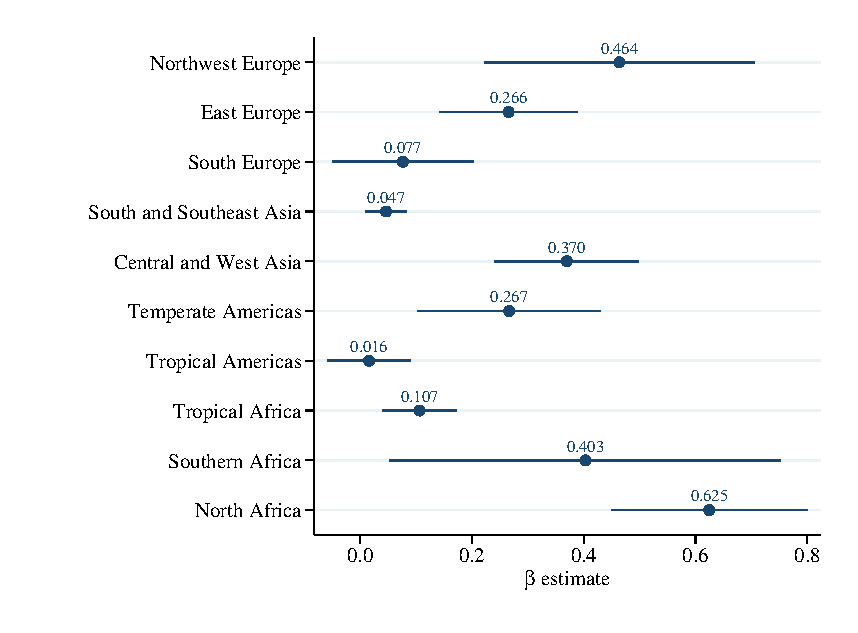
\includegraphics[width=.8\textwidth]{fig_coef_subregion_province.eps}
\end{center}
\hfill \hyperlink{robustness}{\beamerbutton{Return}}
\end{frame}

\begin{frame}{Results by Sub-Region, 2000 CE, Provinces}

{\scriptsize
\begin{tabularx}{\textwidth}{lXXXXX}
\midrule
\multicolumn{6}{l}{Dependent Variable in both panels: Log caloric yield ($A_{isc}$)} \\ \\
\\
Panel A & \multicolumn{5}{c}{Sub-Region:} \\ \cmidrule{2-6}
 &          &         &             &  \multicolumn{2}{c}{Excl. China} \\ \cmidrule(lr){5-6}
 & North \& &         &              & South \&  & Central \&             \\
 & Western  & Eastern & Southern     & Southeast & West        \\
 & Europe   & Europe  & Europe       & Asia      & Asia      \\
 & (1) & (2) & (3) & (4) & (5) \\
\midrule
Log rural density   &       0.464&       0.266&       0.077&       0.047&       0.370\\
                    &     (0.122)&     (0.063)&     (0.064)&     (0.019)&     (0.066)\\
\midrule
p-value $\beta=0$   &       0.000&       0.000&       0.233&       0.013&       0.000\\
p-value $\beta=\beta^{NWEur}$&           .&       0.144&       0.003&       0.001&       0.499\\
Countries           &          16&           9&           9&          13&          18\\
Observations        &         166&         206&         135&         370&         303\\
Adjusted R-square   &        0.40&        0.41&        0.32&        0.35&        0.33\\

\midrule
\end{tabularx}
}

\hfill \hyperlink{robustness}{\beamerbutton{Return}}
\end{frame}

\begin{frame}{Results by Sub-Region, 2000 CE, Provinces}

{\scriptsize
\begin{tabularx}{\textwidth}{lXXXXX}
\midrule
\multicolumn{6}{l}{Dependent Variable in both panels: Log caloric yield ($A_{isc}$)} \\ \\
\\
Panel B & \multicolumn{5}{c}{Sub-Region:} \\ \cmidrule{2-6}
 &           &   &           &          &             \\
 & Temperate & Tropical  & Tropical & South    & North    \\
 & Americas  & Americas  & Africa   & Africa   & Africa     \\
\midrule
Log rural density   &       0.267&       0.016&       0.107&       0.403&       0.625\\
                    &     (0.083)&     (0.038)&     (0.034)&     (0.177)&     (0.089)\\
\midrule
p-value $\beta=0$   &       0.001&       0.670&       0.002&       0.024&       0.000\\
p-value $\beta=\beta^{NWEur}$&       0.184&       0.001&       0.005&       0.778&       0.289\\
Countries           &           5&          20&          39&           4&           5\\
Observations        &          85&         317&         497&          28&          88\\
Adjusted R-square   &        0.34&        0.19&        0.22&        0.39&        0.43\\

\midrule
\end{tabularx}
}

\hfill \hyperlink{robustness}{\beamerbutton{Return}}
\end{frame}

\begin{frame}{Relationship fo $\beta$ to rural density, by province}\label{rurdbeta}
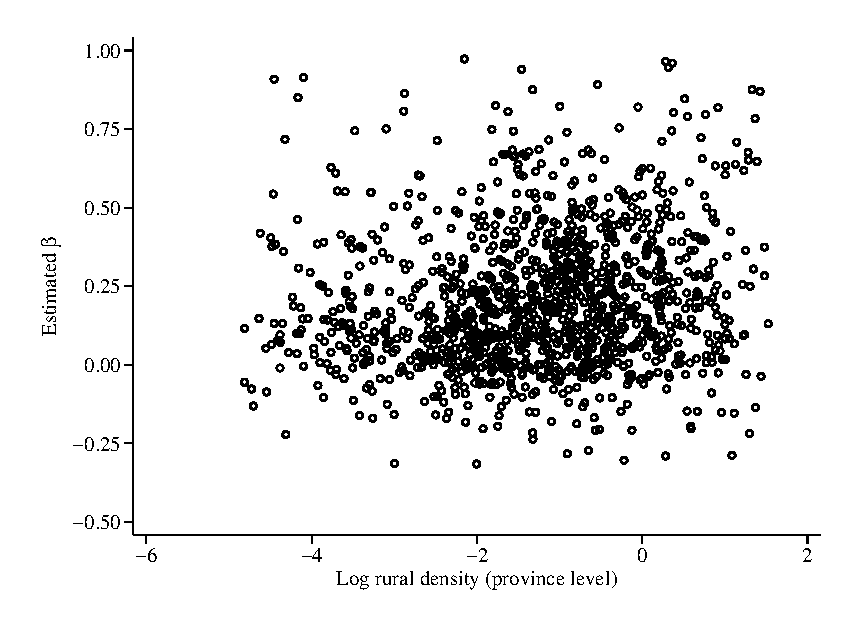
\includegraphics[width=.8\textwidth]{fig_beta_rurd.eps}
\hfill \hyperlink{eos}{\beamerbutton{Return}}
\end{frame}

\begin{frame}{Summary statistics}\label{stats}
{\scriptsize
\begin{tabularx}{\textwidth}{lXXXXXXX}
\midrule
 &      &            & \multicolumn{5}{c}{Percentiles:} \\ \cmidrule{4-8}
 & Mean & SD  & 10th    & 25th    & 50th & 75th & 90th \\
\midrule
Labor/land (persons/ha) &     0.76&     1.19&     0.05&     0.13&     0.34&     0.81&     1.92\\
Caloric yield (mil cals/ha) &    10.83&     4.83&     5.01&     7.20&    10.68&    13.83&    16.93\\
Log light density &    -2.97&     2.92&    -6.43&    -3.93&    -2.63&    -1.03&     0.20\\
Road density (km per sq-km) &     0.40&     0.53&     0.06&     0.11&     0.22&     0.47&     0.90\\
Share of roads, highway &     0.03&     0.09&     0.00&     0.00&     0.00&     0.00&     0.08\\
Share of roads, primary &     0.15&     0.20&     0.00&     0.00&     0.09&     0.22&     0.39\\
Share of roads, secondary &     0.33&     0.30&     0.00&     0.08&     0.24&     0.51&     0.82\\
Slope index &    70.78&    24.18&    33.64&    52.63&    77.69&    91.88&    97.05\\
Distance (km) to city w/ 100,000 &    61.20&    70.57&     6.89&    16.95&    40.33&    78.50&   137.32\\

\midrule
\end{tabularx}
}

\hfill \hyperlink{data}{\beamerbutton{Return}}
\end{frame}

\begin{frame}{Crops used in productivity calculation}\label{crops}
alfalfa, banana, barley, buckwheat, cassava, chickpea, cowpea, drypea, flax, foxtail millet, greengram, groundnut, indica rice, maize, oat, pearl millet, phaselous bean, pigeon pea, rye, sorghum, soybean, spring wheat, sweetpotato, rape, wet/paddy rice, wheat, winter wheat, white potato, and yams

\hfill \hyperlink{data}{\beamerbutton{Return}}
\end{frame}

\begin{frame}{Results by Crop}\label{cropreg}

{\scriptsize
\begin{tabularx}{\textwidth}{lXXXXXX}
\midrule
\multicolumn{7}{l}{Dependent Variable in all panels: Log caloric yield ($A_{isc}$)} \\ \\
\multicolumn{7}{l}{Panel A: Wheat and rice} \\
 & \multicolumn{6}{c}{Inclusion by crop suitability:} \\ \cmidrule(lr){2-7}
 & \multicolumn{4}{c}{Entire world:} & \multicolumn{2}{c}{Ex. Americas:}\\ \cmidrule(lr){2-5} \cmidrule(lr){6-7} 
 & Wheat$>$0& Wheat=0 &         &        & Wheat$>$0   & Wheat=0   \\
 & Rice=0 & Rice$>$0  & Wheat$>$0 & Rice$>$0 & Rice=0    & Rice$>$0   \\
 & (1) & (2) & (3) & (4) & (5) & (6) \\
\midrule
rurd_reg            &       0.227&       0.138\\
                    &     (0.024)&     (0.021)\\
\midrule
p-value $\beta=0$   &       0.000&       0.000\\
p-value $\beta=\beta^{Wheat}$&            &    .0049448\\
Countries           &         106&          74\\
Observations        &    12627.00&    20423.00\\
Adjusted R-square   &        0.21&        0.19\\

\midrule
\end{tabularx}
}

\end{frame}

\begin{frame}{Results by Crop}

{\scriptsize
\begin{tabularx}{\textwidth}{lXXXXXX}
\midrule
\multicolumn{7}{l}{Dependent Variable in all panels: Log caloric yield ($A_{isc}$)} \\ \\
\multicolumn{7}{l}{Panel B: Tropical crops} \\
                   & \multicolumn{6}{c}{Inclusion is wheat suitability = 0, but:} \\ \cmidrule(lr){2-7}
                   &            &              &          &   Pearl       &  Sweet      & \\
& Cassava$>$0 & Cowpea$>$0  & Maize$>$0 & Millet$>$0 & Potato$>$0 & Yams$>$0   \\
\midrule
Log rural density   &       0.140&       0.144&       0.143&       0.154&       0.144&       0.140\\
                    &     (0.021)&     (0.020)&     (0.020)&     (0.019)&     (0.020)&     (0.020)\\
\midrule
p-value $\beta=0$   &       0.000&       0.000&       0.000&       0.000&       0.000&       0.000\\
Countries           &          74&          80&          78&          72&          77&          78\\
Observations        &        8052&        8312&        8377&        6590&        8354&        8269\\
Adjusted R-square   &        0.13&        0.13&        0.13&        0.13&        0.13&        0.12\\

\midrule
\end{tabularx}
}

\end{frame}

\begin{frame}{Results by Crop}

{\scriptsize
\begin{tabularx}{\textwidth}{lXXXXXX}
\midrule
\multicolumn{7}{l}{Dependent Variable in all panels: Log caloric yield ($A_{isc}$)} \\ \\
\multicolumn{7}{l}{Panel C: Temperate crops} \\
                   & \multicolumn{6}{c}{Inclusion is rice suitability = 0, but:} \\ \cmidrule(lr){2-7}
                   &            & Buck-        &          &          &         & White \\
                   & Barley$>$0 & wheat$>$0  & Oats$>$0 & Flax$>$0 & Rye$>$0 & Potato$>$0   \\
\midrule
Log rural density   &       0.227&       0.228&       0.234&       0.228&       0.235&       0.227\\
                    &     (0.024)&     (0.025)&     (0.025)&     (0.025)&     (0.025)&     (0.023)\\
\midrule
p-value $\beta=0$   &       0.000&       0.000&       0.000&       0.000&       0.000&       0.000\\
Countries           &         106&          76&          72&          74&          72&         105\\
Observations        &       12627&       11162&       11089&       11035&       11106&       12494\\
Adjusted R-square   &        0.21&        0.23&        0.23&        0.23&        0.23&        0.22\\

\midrule
\end{tabularx}
}

\hfill \hyperlink{crop}{\beamerbutton{Plot}}
\end{frame}


\begin{frame}{Results by Province}\label{prov}
Regions and sub-regions assume $\beta$ constant within region/sub-region. 

\vspace{.2cm}Instead, estimate $\beta$ individually for each province
\begin{itemize}
  \item Only provinces with 6 or more districts (1,340 provinces)
  \item ... so really big SE on any individual estimate
  \item Look at pattern of $\beta$'s for each sub-region
\end{itemize}
\end{frame}

\begin{frame}{Results by Province}
\begin{center}
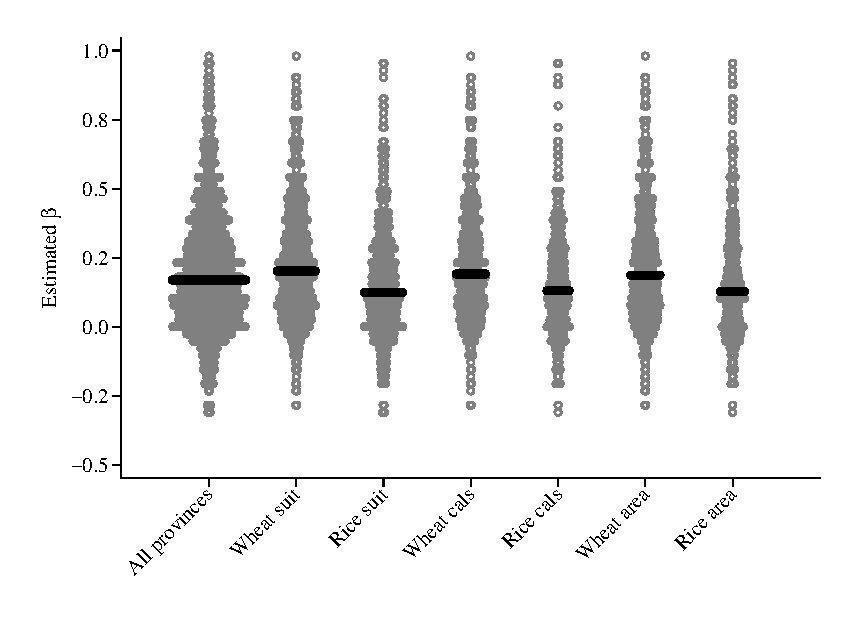
\includegraphics[width=.8\textwidth]{fig_beta_province.eps}
\end{center}
\end{frame}

\begin{frame}{Results by Province}

{\tiny
\begin{tabularx}{\textwidth}{lrXrXrXrXrXrXrXr}
\midrule
           &       &&      &&     && \multicolumn{9}{c}{Percentiles:} \\ \cmidrule{8-16}
Sub-region & Prov. && Mean && SD  && 10th    && 25th    && 50th && 75th && 90th \\
\midrule
All provinces &    1,260&     0.21&     0.31&    -0.04&     0.04&     0.17&     0.33&     0.52\\
Wheat Suitable &      640&     0.24&     0.25&    -0.01&     0.08&     0.21&     0.38&     0.55\\
Rice Suitable &      514&     0.16&     0.28&    -0.06&     0.01&     0.12&     0.28&     0.45\\
Wheat cals>33\% &      484&     0.23&     0.26&    -0.01&     0.08&     0.19&     0.37&     0.55\\
Rice cals>33\% &      328&     0.16&     0.23&    -0.06&     0.02&     0.13&     0.28&     0.41\\
Wheat area>50\% &      511&     0.24&     0.27&    -0.01&     0.07&     0.19&     0.37&     0.55\\
Rice area>50\% &      315&     0.17&     0.26&    -0.06&     0.00&     0.12&     0.29&     0.50\\

\midrule
\end{tabularx}
}

\hfill \hyperlink{robustness}{\beamerbutton{Return}}
\end{frame}


\begin{frame}{Labor and capital not mobile}\label{nonmobile}
Factors cannot move within province, but output can.

\vspace{.2cm} Changes relationship of density and productivity to
\begin{equation}
  \ln A_{Ai} = \beta \ln L_{Ai}/X_i + \ln A_{Ni} + \alpha\beta \ln K_i/L_i + \ln p_N/p_A \nonumber
\end{equation}
\begin{itemize}
  \item Night lights provide proxy for $A_{Ni}$ and $K_i/L_i$?
  \item $p_N/p_A$ is province-specific (FE)
  \item Is correlation of $A_{Ni}$ and $K_i/L_i$ with $L_{Ai}/X_i$ different by climate zone?
\end{itemize}

\hfill \hyperlink{robustness}{\beamerbutton{Return}}
\end{frame}

\begin{frame}{Districts are autarkic}\label{autarky}
Factors and output are immobile within province.

\vspace{.2cm} Changes relationship of density and productivity to
\begin{equation}
\ln A_i = \beta \ln L_{Ai}/X_i - \ln L_{A_i}/L_i - \alpha(1-\beta) \ln K_{i}/L_{i} + \ln c_{Ai} \nonumber
\end{equation}
\begin{itemize}
  \item Can control for $L_{Ai}/L_i$ using HYDE data
  \item Night lights provide proxy for $K_i/L_i$?
  \item $c_{Ai}$ doesn't vary much and/or proxied by night lights?
\end{itemize}

\end{frame}

\begin{frame}{Results controlling for $\ln L_{Ai}/L_i$}
\begin{center}
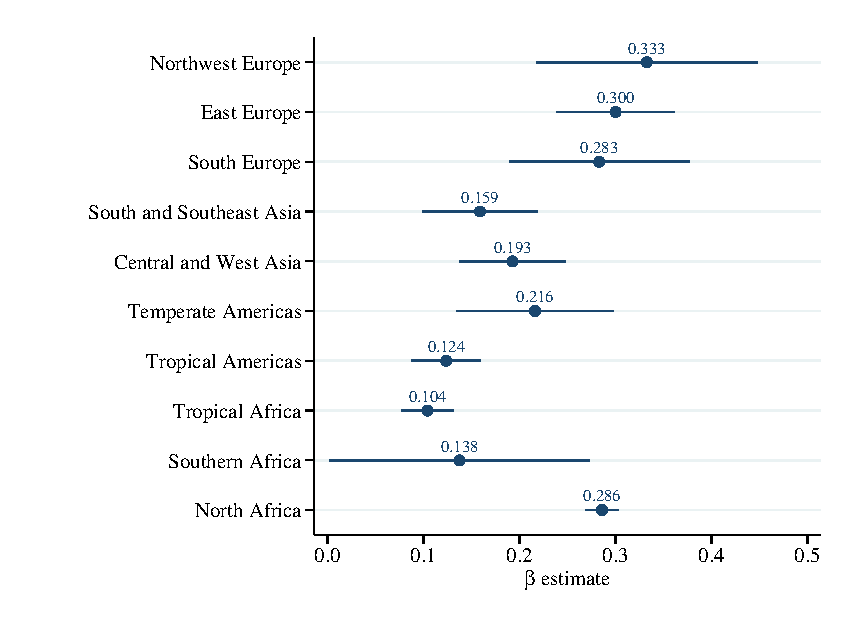
\includegraphics[width=.8\textwidth]{fig_coef_subregion_autarky.eps}
\end{center}
\hfill \hyperlink{robustness}{\beamerbutton{Return}}
\end{frame}

\begin{frame}{Results controlling for $\ln L_{Ai}/L_i$}

{\scriptsize
\begin{tabularx}{\textwidth}{lXXXXX}
\midrule
\multicolumn{6}{l}{Dependent Variable in both panels: Log caloric yield ($A_{isc}$)} \\ \\
\\
Panel A & \multicolumn{5}{c}{Sub-Region:} \\ \cmidrule{2-6}
 &          &         &             &  \multicolumn{2}{c}{Excl. China} \\ \cmidrule(lr){5-6}
 & North \& &         &              & South \&  & Central \&             \\
 & Western  & Eastern & Southern     & Southeast & West        \\
 & Europe   & Europe  & Europe       & Asia      & Asia      \\
 & (1) & (2) & (3) & (4) & (5) \\
\midrule
Log rural density   &       0.333&       0.300&       0.283&       0.159&       0.193\\
                    &     (0.059)&     (0.031)&     (0.048)&     (0.031)&     (0.028)\\
\midrule
p-value $\beta=0$   &       0.000&       0.000&       0.000&       0.000&       0.000\\
p-value $\beta=\beta^{NWEur}$&           .&       0.617&       0.460&       0.009&       0.031\\
Countries           &          16&           9&           9&          13&          18\\
Observations        &        1628&        4772&        1114&        3921&        2762\\
Adjusted R-square   &        0.28&        0.33&        0.31&        0.20&        0.21\\

\midrule
\end{tabularx}
}

\end{frame}

\begin{frame}{Results controlling for $\ln L_{Ai}/L_i$}

{\scriptsize
\begin{tabularx}{\textwidth}{lXXXXX}
\midrule
\multicolumn{6}{l}{Dependent Variable in both panels: Log caloric yield ($A_{isc}$)} \\ \\
\\
Panel B & \multicolumn{5}{c}{Sub-Region:} \\ \cmidrule{2-6}
 &           &   &           &          &             \\
 & Temperate & Tropical  & Tropical & South    & North    \\
 & Americas  & Americas  & Africa   & Africa   & Africa     \\
\midrule
Log rural density   &       0.216&       0.124&       0.104&       0.138&       0.286\\
                    &     (0.042)&     (0.018)&     (0.014)&     (0.069)&     (0.009)\\
\midrule
p-value $\beta=0$   &       0.000&       0.000&       0.000&       0.047&       0.000\\
p-value $\beta=\beta^{NWEur}$&       0.105&       0.001&       0.000&       0.032&       0.431\\
Countries           &           5&          22&          39&           4&           5\\
Observations        &        3183&        8730&        3032&         178&        1147\\
Adjusted R-square   &        0.22&        0.11&        0.18&        0.25&        0.28\\

\midrule
\end{tabularx}
}
\end{frame}

\begin{frame}{Results for China, Japan, Korea}\label{chinareg}

{\scriptsize
\begin{tabularx}{\textwidth}{lXXXXX}
\midrule
\multicolumn{4}{l}{Dependent Variable: Log caloric yield ($A_{isc}$)} \\
 & All& Temperate & Sub-Trop & & N. \& \\
 & China & China  & China & Japan & S. Korea  \\
 & (1) & (2) & (3) & (4) & (5) \\
\midrule
Residuals           &       0.414&       0.518&       0.107&       0.155&       0.190\\
                    &     (0.089)&     (0.060)&     (0.021)&     (0.003)&     (0.060)\\
\midrule
p-value $\beta=0$   &       0.000&       0.000&       0.000&       0.000&       0.002\\
p-value $\beta=\beta^{Temp}$&            &            &       0.000&            &            \\
Observations        &         266&         130&         136&        1039&         311\\
Adjusted R-square   &        0.56&        0.70&        0.13&        0.23&        0.23\\

\midrule
\end{tabularx}
}

\hfill \hyperlink{china}{\beamerbutton{Plot}}
\end{frame}

\begin{frame}{Results by Major Region}\label{regiontab}

{\scriptsize
\begin{tabularx}{\textwidth}{lXXXXXX}
\midrule
\multicolumn{7}{l}{Dependent Variable: Log caloric yield ($A_{isc}$)} \\
 & \multicolumn{6}{c}{Region:} \\ \cmidrule{2-7}
 &        & East \& & Sub-        & North     & South \&  &  \\
 &        & South   & Saharan     & Africa \& & Central   & U.S. and \\
 & Europe & Asia    & Africa      & West Asia & America   & Canada \\
 & (1) & (2) & (3) & (4) & (5) & (6) \\
\midrule
\input{tab_beta_region_gadm2_2000_spatial.tex}
\midrule
\end{tabularx}
}

\hfill \hyperlink{region}{\beamerbutton{Plot}}
\end{frame}

\begin{frame}{Results by Sub-Region}\label{subregiontab}

{\scriptsize
\begin{tabularx}{\textwidth}{lXXXXX}
\midrule
\multicolumn{6}{l}{Dependent Variable in both panels: Log caloric yield ($A_{isc}$)} \\ \\
\\
Panel A & \multicolumn{5}{c}{Sub-Region:} \\ \cmidrule{2-6}
 &          &         &             &  \multicolumn{2}{c}{Excl. China} \\ \cmidrule(lr){5-6}
 & North \& &         &              & South \&  & Central \&             \\
 & Western  & Eastern & Southern     & Southeast & West        \\
 & Europe   & Europe  & Europe       & Asia      & Asia      \\
 & (1) & (2) & (3) & (4) & (5) \\
\midrule
\input{tab_beta_subregionA_gadm2_2000_spatial.tex}
\midrule
\end{tabularx}
}
\end{frame}

\begin{frame}{Results by Sub-Region}

{\scriptsize
\begin{tabularx}{\textwidth}{lXXXXX}
\midrule
\multicolumn{6}{l}{Dependent Variable in both panels: Log caloric yield ($A_{isc}$)} \\ \\
\\
Panel B & \multicolumn{5}{c}{Sub-Region:} \\ \cmidrule{2-6}
 &           &   &           &          &             \\
 & Temperate & Tropical  & Tropical & South    & North    \\
 & Americas  & Americas  & Africa   & Africa   & Africa     \\
\midrule
\input{tab_beta_subregionB_gadm2_2000_spatial.tex}
\midrule
\end{tabularx}
}

\hfill \hyperlink{subregion}{\beamerbutton{Plot}}
\end{frame}


\begin{frame}{Results by Climate Zone}\label{climatereg}

{\scriptsize
\begin{tabularx}{\textwidth}{lXXXXXX}
\midrule
\multicolumn{7}{l}{Dependent Variable in all panels: Log caloric yield ($A_{isc}$)} \\ \\
\multicolumn{7}{l}{Panel A: Climate Zones} \\
 & Equatorial & Arid  & Temperate & Snow &     &   \\
 & (1) & (2) & (3) & (4) &  & \\
\midrule
Log rural density   &       0.118&       0.154&       0.171&       0.237\\
                    &     (0.018)&     (0.034)&     (0.024)&     (0.031)\\
\midrule
p-value $\beta=0$   &       0.000&       0.000&       0.000&       0.000\\
Countries           &          81&          57&          94&          43\\
Observations        &       10752&        2675&       13019&        6058\\
Adjusted R-square   &        0.11&        0.09&        0.17&        0.27\\

\midrule
\end{tabularx}
}

\end{frame}

\begin{frame}{Results by Precipitation Zone}

{\scriptsize
\begin{tabularx}{\textwidth}{lXXXXXX}
\midrule
\multicolumn{7}{l}{Panel B: Precipitation Zones} \\
& Fully     & Dry         & Dry        &              &            & \\
& Humid & Summer  & Winter & Monsoons & Desert & Steppe   \\
 & (1) & (2) & (3) & (4) & (5) & (6) \\
\midrule
Log rural density   &       0.187&       0.183&       0.127&       0.135&       0.109&       0.116\\
                    &     (0.033)&     (0.030)&     (0.021)&     (0.029)&     (0.039)&     (0.031)\\
\midrule
p-value $\beta=0$   &       0.000&       0.000&       0.000&       0.000&       0.005&       0.000\\
Countries           &          99&          46&          75&          43&          34&          55\\
Observations        &       16371&        3067&        8683&        1729&         390&        2270\\
Adjusted R-square   &        0.19&        0.19&        0.12&        0.12&        0.04&        0.06\\

\midrule
\end{tabularx}
}

\end{frame}

\begin{frame}{Results by Temperature Zone}

{\scriptsize
\begin{tabularx}{\textwidth}{lXXXXXX}
\midrule
\multicolumn{7}{l}{Panel C: Temperature Zones} \\
    & Hot        & Warm        & Cool       & Hot      & Cold     &  \\
    & Summer & Summer  & Summer & Arid & Arid &   \\
 & (1) & (2) & (3) & (4) & (5) &  \\    
\midrule
Log rural density   &       0.141&       0.227&       0.254&       0.135&       0.142\\
                    &     (0.020)&     (0.034)&     (0.047)&     (0.032)&     (0.045)\\
\midrule
p-value $\beta=0$   &       0.000&       0.000&       0.000&       0.000&       0.002\\
Countries           &          61&          86&          26&          45&          26\\
Observations        &        8749&        9751&         487&        1594&        1065\\
Adjusted R-square   &        0.15&        0.25&        0.13&        0.07&        0.09\\

\midrule
\end{tabularx}
}

\hfill \hyperlink{climate}{\beamerbutton{Plot}}
\end{frame}


\begin{frame}{Results using Cultivated Area}\label{cultreg}
\begin{center}
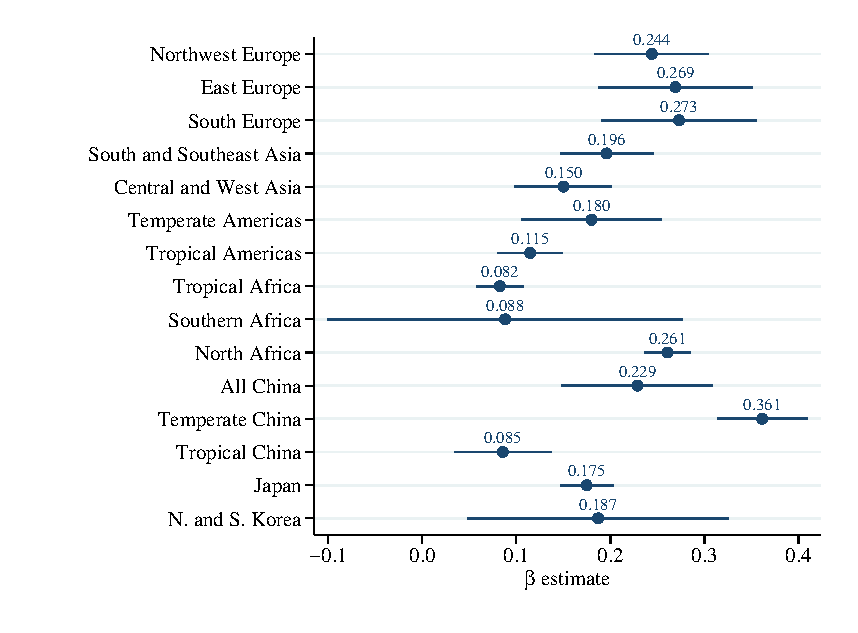
\includegraphics[width=.8\textwidth]{fig_coef_subregion_cult.eps}
\end{center}
\hfill \hyperlink{cult}{\beamerbutton{Return}}
\end{frame}

\begin{frame}{Results using Cultivated Area}

{\scriptsize
\begin{tabularx}{\textwidth}{lXXXXX}
\midrule
\multicolumn{6}{l}{Dependent Variable in both panels: Log caloric yield ($A_{isc}$)} \\ \\
\\
Panel A & \multicolumn{5}{c}{Sub-Region:} \\ \cmidrule{2-6}
 &          &         &             &  \multicolumn{2}{c}{Excl. China} \\ \cmidrule(lr){5-6}
 & North \& &         &              & South \&  & Central \&             \\
 & Western  & Eastern & Southern     & Southeast & West        \\
 & Europe   & Europe  & Europe       & Asia      & Asia      \\
 & (1) & (2) & (3) & (4) & (5) \\
\midrule
\input{tab_beta_subregionA_spatial_cult.tex}
\midrule
\end{tabularx}
}

\end{frame}

\begin{frame}{Results using Cultivated Area}

{\scriptsize
\begin{tabularx}{\textwidth}{lXXXXX}
\midrule
\multicolumn{6}{l}{Dependent Variable in both panels: Log caloric yield ($A_{isc}$)} \\ \\
\\
Panel B & \multicolumn{5}{c}{Sub-Region:} \\ \cmidrule{2-6}
 &           &   &           &          &             \\
 & Temperate & Tropical  & Tropical & South    & North    \\
 & Americas  & Americas  & Africa   & Africa   & Africa     \\
\midrule
Log rural density   &       0.180&       0.115&       0.082&       0.088&       0.261\\
                    &     (0.038)&     (0.018)&     (0.013)&     (0.096)&     (0.012)\\
\midrule
p-value $\beta=0$   &       0.000&       0.000&       0.000&       0.361&       0.000\\
p-value $\beta=\beta^{NWEur}$&       0.189&       0.000&       0.000&       0.123&       0.620\\
Countries           &           5&          22&          39&           4&           5\\
Observations        &        3183&        8696&        2976&         171&        1134\\
Adjusted R-square   &        0.16&        0.09&        0.12&        0.16&        0.21\\

\midrule
\end{tabularx}
}

\end{frame}

\end{document}
